\chapter{Thiết kế phần mềm}

\section{Tổng quan thiết kế phần mềm}

Thiết kế phần mềm của hệ thống được chia thành ba phần: thiết kế dữ liệu, thiết kế xử lý và thiết kế giao diện. Thiết kế dữ liệu mô tả cách hệ thống lưu trữ và ràng buộc dữ liệu; thiết kế xử lý mô tả luồng nghiệp vụ, API và business rules; thiết kế giao diện mô tả cách người dùng tương tác với hệ thống.

\section{Nguyên tắc thiết kế phần mềm}

Thiết kế phần mềm của hệ thống được xây dựng dựa trên các yêu cầu đã đặc tả ở Chương 1 và kiến trúc hệ thống ở Chương 2. Vì đây là một hệ thống thông tin nghiệp vụ cho phòng mạch tư nhân, thiết kế cần ưu tiên tính rõ ràng của dữ liệu, tính nhất quán của luồng xử lý và khả năng truy vết từ yêu cầu đến hiện thực.

\begin{longtable}{|p{4cm}|p{10.5cm}|}
\caption{Nguyên tắc thiết kế phần mềm}\\
\hline
\textbf{Nguyên tắc} & \textbf{Ý nghĩa áp dụng trong hệ thống} \\
\hline
Lấy nghiệp vụ làm trung tâm & Các model, service và màn hình được tổ chức quanh các nghiệp vụ chính như bệnh nhân, lượt khám, phiếu khám, hóa đơn, thanh toán, xét nghiệm và cấp phát thuốc. \\
\hline
Tách dữ liệu lõi và dữ liệu mở rộng & Patient, Visit, Examination, Prescription, Invoice và Payment là lõi Phase 1; Appointment, Queue, Lab, Inventory và Pharmacy là phần mở rộng Phase 2. \\
\hline
Đặt business rules ở backend service layer & Frontend chỉ hỗ trợ trải nghiệm người dùng; các quy tắc như chống trùng lượt khám, không thanh toán vượt số tiền còn lại hoặc FEFO phải được kiểm soát ở backend. \\
\hline
Ưu tiên toàn vẹn dữ liệu & Các nghiệp vụ nhiều bảng như tạo lượt khám, hoàn tất khám, lập hóa đơn, thanh toán và cấp phát thuốc cần transaction hoặc ràng buộc dữ liệu phù hợp. \\
\hline
Bảo toàn dữ liệu lịch sử & Các thông tin như giá thuốc, phí khám, invoice item, quy định và kết quả xét nghiệm cần được lưu theo thời điểm phát sinh để tránh thay đổi lịch sử khi danh mục hiện tại thay đổi. \\
\hline
Dễ truy vết và kiểm thử & Mỗi yêu cầu quan trọng cần truy được sang model, API, service, màn hình và test case tương ứng. \\
\hline
\end{longtable}

\noindent
Các đầu vào chính của thiết kế phần mềm gồm: danh sách yêu cầu chức năng, yêu cầu phi chức năng, use case, business rules, kiến trúc client--server, quyết định modular monolith, Prisma schema, các module backend/frontend và các luồng demo trọng tâm. Nhờ đó, Chương 3 đóng vai trò cầu nối giữa đặc tả yêu cầu và hiện thực mã nguồn.

\subsection{Cách đọc ERD và phạm vi sơ đồ}

Do hệ thống có nhiều nhóm nghiệp vụ, ERD được tách thành hai phần để tránh sơ đồ quá lớn và khó đọc. ERD Phase 1 mô tả các entity lõi phục vụ quy trình tiếp nhận, khám bệnh, kê đơn, lập hóa đơn và thanh toán. ERD Phase 2 Delta mô tả các entity mở rộng như lịch hẹn, hàng đợi, sinh hiệu, dịch vụ, xét nghiệm, kho thuốc và cấp phát thuốc.

\begin{table}[H]
\centering
\caption{Phạm vi các sơ đồ ERD trong báo cáo}
\begin{tabularx}{\textwidth}{|p{4cm}|X|}
\hline
\textbf{Sơ đồ} & \textbf{Nội dung chính} \\
\hline
ERD Phase 1 & User, Role, Permission, Patient, Visit, Examination, Diagnosis, Disease, Prescription, PrescriptionItem, Drug, Invoice, InvoiceItem, Payment, RegulationVersion và RegulationItem. \\
\hline
ERD Phase 2 Delta & Appointment, QueueTicket, VitalSign, ServiceCatalog, LabTestCatalog, ServiceOrder, LabOrder, LabSample, LabResult, StockLot, StockMovement, Dispense, DispenseItem, Department, Room, DoctorProfile và StaffSchedule. \\
\hline
\end{tabularx}
\end{table}

\noindent
Cách tách này giúp báo cáo vừa thể hiện được đầy đủ phạm vi hệ thống, vừa giữ được khả năng đọc hiểu. Khi bảo vệ, có thể trình bày Phase 1 trước để chứng minh baseline nghiệp vụ lõi, sau đó trình bày Phase 2 như phần mở rộng quanh lõi Patient--Visit--Examination--Billing.

\subsection{Quan hệ và multiplicity giữa các entity lõi}

Bảng dưới đây mô tả các quan hệ quan trọng giữa các entity lõi. Phần này bổ sung cho ERD bằng cách giải thích rõ ý nghĩa nghiệp vụ của từng quan hệ thay vì chỉ dựa vào hình.

\begin{longtable}{|p{4.2cm}|p{3cm}|p{7cm}|}
\caption{Quan hệ dữ liệu lõi và ý nghĩa nghiệp vụ}\\
\hline
\textbf{Quan hệ} & \textbf{Bội số} & \textbf{Ý nghĩa thiết kế} \\
\hline
Patient -- Visit & 1 -- 0..* & Một bệnh nhân có thể có nhiều lượt khám theo thời gian; Visit là điểm bắt đầu của quy trình khám trong ngày. \\
\hline
Visit -- Examination & 1 -- 0..1 & Một lượt khám có tối đa một phiếu khám chính; phiếu khám chỉ có ý nghĩa trong ngữ cảnh một visit cụ thể. \\
\hline
Examination -- Diagnosis & 1 -- 0..* & Một phiếu khám có thể có nhiều chẩn đoán; hệ thống cần kiểm soát tối đa một chẩn đoán chính. \\
\hline
Diagnosis -- Disease & 0..* -- 0..1 & Diagnosis có thể tham chiếu danh mục bệnh chuẩn, nhưng vẫn nên lưu thông tin tại thời điểm khám nếu cần bảo toàn lịch sử. \\
\hline
Examination -- Prescription & 1 -- 0..1 & Một phiếu khám có thể không kê đơn hoặc có một đơn thuốc chính. \\
\hline
Prescription -- PrescriptionItem & 1 -- 1..* & Một đơn thuốc gồm nhiều dòng thuốc; PrescriptionItem phụ thuộc vòng đời vào Prescription. \\
\hline
PrescriptionItem -- Drug & 0..* -- 1 & Mỗi dòng thuốc tham chiếu một thuốc trong danh mục; cần lưu snapshot giá/thông tin cần thiết để bảo toàn dữ liệu quá khứ. \\
\hline
Visit -- Invoice & 1 -- 0..1 & Một lượt khám có tối đa một hóa đơn chính trong phạm vi Phase 1, tránh phát sinh hóa đơn trùng. \\
\hline
Invoice -- InvoiceItem & 1 -- 1..* & Một hóa đơn gồm nhiều dòng phí như phí khám, thuốc hoặc dịch vụ. \\
\hline
Invoice -- Payment & 1 -- 0..* & Một hóa đơn có thể được thanh toán một lần hoặc nhiều lần, hỗ trợ trạng thái PARTIALLY\_PAID và PAID. \\
\hline
Drug -- StockLot & 1 -- 0..* & Một thuốc có thể có nhiều lô tồn kho với hạn dùng khác nhau, phục vụ FEFO ở Phase 2. \\
\hline
Prescription -- Dispense & 1 -- 0..1 & Một đơn thuốc có thể được cấp phát một lần theo quy trình Pharmacy nếu module Phase 2 được dùng. \\
\hline
\end{longtable}


\section{Thiết kế dữ liệu}

\subsection{Mục tiêu thiết kế dữ liệu}

Cơ sở dữ liệu được thiết kế nhằm đảm bảo dữ liệu bệnh nhân, lượt khám, phiếu khám, đơn thuốc, hóa đơn, thanh toán, lịch hẹn, xét nghiệm và kho thuốc được lưu trữ nhất quán. Hệ thống sử dụng PostgreSQL và Prisma ORM. Schema hiện có 37 models, 12 enums và 3 migrations.
\subsection{ERD tổng thể và cách tách sơ đồ}
\ReportFigure{figures/ch03-software-design/erd-phase1.pdf}{ERD Phase 1 -- nghiệp vụ lõi phòng mạch}{fig:erd-phase1}
\ReportFigure{figures/ch03-software-design/erd-phase2-delta.pdf}{ERD Phase 2 Delta -- các model mở rộng}{fig:erd-phase2-delta}

\subsection{Các nhóm model chính}

\begin{longtable}{|p{3.3cm}|p{5.5cm}|p{5.4cm}|}
\caption{Các nhóm model trong cơ sở dữ liệu}\\
\hline
\textbf{Nhóm} & \textbf{Models} & \textbf{Vai trò thiết kế} \\
\hline
Identity \& Access & User, Role, Permission, UserRole, RolePermission, RefreshToken, AuditLog & Quản lý tài khoản, vai trò, quyền, token và nhật ký hệ thống \\
\hline
Patients \& Visits & Patient, Visit & Quản lý hồ sơ bệnh nhân, lượt khám và số thứ tự \\
\hline
Examination \& Prescription & Examination, Disease, Diagnosis, Drug, Prescription, PrescriptionItem & Lưu phiếu khám, chẩn đoán, danh mục bệnh, thuốc và đơn thuốc \\
\hline
Billing \& Regulation & Invoice, InvoiceItem, Payment, RegulationVersion, RegulationItem & Quản lý hóa đơn, thanh toán và quy định phòng mạch \\
\hline
Organization & Department, Room, DoctorProfile, StaffSchedule & Quản lý tổ chức phòng khám, phòng và bác sĩ \\
\hline
Appointment \& Queue & Appointment, QueueTicket & Quản lý lịch hẹn và hàng đợi \\
\hline
Vitals \& Services \& Lab & VitalSign, ServiceCatalog, LabTestCatalog, ServiceOrder, LabOrder, LabSample, LabResult & Sinh hiệu, chỉ định dịch vụ và quy trình xét nghiệm \\
\hline
Inventory \& Pharmacy & StockLot, StockMovement, Dispense, DispenseItem & Quản lý tồn kho, biến động kho và cấp phát thuốc \\
\hline
\end{longtable}

\subsection{Enum và state machine}

\begin{longtable}{|p{4cm}|p{8cm}|p{3cm}|}
\caption{Danh sách 12 enum trong database}\\
\hline
\textbf{Enum} & \textbf{Values} & \textbf{Model sử dụng} \\
\hline
UserStatus & ACTIVE, INACTIVE, LOCKED & User \\
\hline
VisitStatus & REGISTERED, WAITING, IN\_EXAMINATION, COMPLETED, CANCELLED & Visit \\
\hline
ExaminationStatus & OPEN, COMPLETED, CANCELLED & Examination \\
\hline
InvoiceStatus & DRAFT, ISSUED, PARTIALLY\_PAID, PAID, VOID & Invoice \\
\hline
PaymentMethod & CASH, TRANSFER, CARD & Payment \\
\hline
AppointmentStatus & SCHEDULED, CHECKED\_IN, CANCELLED, NO\_SHOW & Appointment \\
\hline
QueueStatus & WAITING, CALLED, IN\_SERVICE, DONE, SKIPPED, CANCELLED & QueueTicket \\
\hline
ServiceType & CONSULTATION, LAB\_TEST, PROCEDURE & ServiceCatalog \\
\hline
DispenseStatus & PENDING, DISPENSED, CANCELLED & Dispense \\
\hline
StockMovementType & IN, OUT, ADJUSTMENT & StockMovement \\
\hline
LabOrderStatus & ORDERED, SAMPLE\_COLLECTED, RESULT\_ENTERED, VERIFIED, CANCELLED & LabOrder \\
\hline
ServiceOrderStatus & ORDERED, IN\_PROGRESS, COMPLETED, CANCELLED & ServiceOrder \\
\hline
\end{longtable}

\begin{longtable}{|p{2.6cm}|p{3.5cm}|p{4.8cm}|p{3.4cm}|}
\caption{Chuyển trạng thái các entity lõi trong hệ thống}\label{tab:state-transitions}\\
\hline
\textbf{Entity} & \textbf{Trạng thái hiện tại} & \textbf{Sự kiện kích hoạt} & \textbf{Trạng thái mới} \\
\hline
\multicolumn{4}{|l|}{\textbf{Visit}} \\
\hline
Visit & -- & Lễ tân tạo lượt khám & WAITING \\
\hline
Visit & WAITING & Bác sĩ mở phiên khám & IN\_\allowbreak EXAMINATION \\
\hline
Visit & IN\_\allowbreak EXAMINATION & Phiếu khám hoàn tất & COMPLETED \\
\hline
Visit & WAITING / IN\_\allowbreak EXAMINATION & Hủy lượt khám & CANCELLED \\
\hline
\multicolumn{4}{|l|}{\textbf{Examination}} \\
\hline
Examination & -- & Bác sĩ mở phiên khám & OPEN \\
\hline
Examination & OPEN & Hoàn tất phiếu khám & COMPLETED \\
\hline
Examination & OPEN & Hủy & CANCELLED \\
\hline
\multicolumn{4}{|l|}{\textbf{Invoice}} \\
\hline
Invoice & -- & Thu ngân lập hóa đơn & ISSUED \\
\hline
Invoice & ISSUED & Thanh toán chưa đủ & PARTIALLY\_PAID \\
\hline
Invoice & ISSUED / PARTIALLY\_PAID & Thanh toán đủ số tiền & PAID \\
\hline
Invoice & ISSUED / PARTIALLY\_PAID & Hủy hóa đơn & VOID \\
\hline
\multicolumn{4}{|l|}{\textbf{QueueTicket (Phase 2)}} \\
\hline
QueueTicket & -- & Check-in tạo vé hàng đợi & WAITING \\
\hline
QueueTicket & WAITING & Gọi tên bệnh nhân & CALLED \\
\hline
QueueTicket & CALLED & Bắt đầu phục vụ & IN\_SERVICE \\
\hline
QueueTicket & IN\_SERVICE & Hoàn tất & DONE \\
\hline
QueueTicket & WAITING / CALLED & Hủy hoặc bỏ qua & CANCELLED \\
\hline
\end{longtable}

Bảng~\ref{tab:state-transitions} tóm tắt các chuyển trạng thái được phép trong quy trình vận hành. Ví dụ, \code{VisitStatus} đi từ WAITING sang IN\_EXAMINATION khi bác sĩ mở phiên khám, sau đó sang COMPLETED khi phiếu khám hoàn tất; các trạng thái CANCELLED/VOID chỉ được dùng cho luồng hủy hoặc vô hiệu hóa có kiểm soát. Việc định nghĩa rõ chuyển trạng thái giúp backend tránh cập nhật tùy tiện và giúp frontend hiển thị hành động phù hợp theo từng trạng thái.

\subsection{Ràng buộc dữ liệu quan trọng}

\begin{longtable}{|p{5.2cm}|p{3.2cm}|p{6cm}|}
\caption{Ràng buộc dữ liệu quan trọng}\\
\hline
\textbf{Ràng buộc} & \textbf{Model} & \textbf{Ý nghĩa} \\
\hline
UUID primary key & Tất cả model & Không dùng serial integer, giảm khả năng đoán ID \\
\hline
\code{patientCode @unique} & Patient & Mỗi bệnh nhân có mã riêng \\
\hline
\code{citizenId @unique} & Patient & Tránh trùng định danh bệnh nhân \\
\hline
\code{@@unique([patientId, visitDate])} & Visit & Ngăn một bệnh nhân có hai lượt khám trong cùng ngày \\
\hline
\code{@@unique([visitDate, queueNumber])} & Visit & Số thứ tự không trùng trong ngày \\
\hline
\code{visitId @unique} & Examination, Invoice & Một lượt khám có một phiếu khám và một hóa đơn chính \\
\hline
\code{examinationId @unique} & Prescription & Một phiếu khám có tối đa một đơn thuốc \\
\hline
\texttt{@@unique([}\newline\texttt{prescriptionId,}\newline\texttt{drugId])} & PrescriptionItem & Không kê trùng cùng một thuốc trong một đơn \\
\hline
\code{@@unique([drugId, lotNumber])} & StockLot & Không trùng mã lô cho cùng một thuốc \\
\hline
\end{longtable}

\subsection{Quyết định thiết kế dữ liệu}

\begin{table}[H]
\centering
\caption{Các quyết định thiết kế dữ liệu quan trọng}
\begin{tabularx}{\textwidth}{|p{4cm}|X|}
\hline
\textbf{Quyết định} & \textbf{Lý do} \\
\hline
Dùng UUID làm primary key & Phù hợp khi hệ thống mở rộng, không để lộ thứ tự tăng dần của bản ghi \\
\hline
Soft-delete bằng \code{isActive} & Giữ lịch sử đối với Disease, Drug, ServiceCatalog thay vì xóa cứng \\
\hline
Snapshot giá trong PrescriptionItem & Lưu đơn giá tại thời điểm kê đơn, tránh thay đổi lịch sử khi giá thuốc thay đổi \\
\hline
RegulationVersion + RegulationItem & Cho phép quản lý phiên bản quy định và chỉ kích hoạt một phiên bản tại một thời điểm \\
\hline
StockLot + StockMovement & Phục vụ quản lý tồn kho, hạn dùng và audit biến động kho \\
\hline
\end{tabularx}
\end{table}

\section{Thiết kế lớp và module nghiệp vụ}

Bên cạnh thiết kế dữ liệu, hệ thống cần có thiết kế lớp và module để mô tả cách các đối tượng nghiệp vụ và service phối hợp với nhau. Trong codebase NestJS, các lớp domain được ánh xạ chủ yếu qua Prisma models, còn logic nghiệp vụ được hiện thực trong các service. Do đó, thiết kế lớp của hệ thống được trình bày theo hai góc nhìn: nhóm entity nghiệp vụ và nhóm service điều phối use case.

\subsection{Nhóm entity nghiệp vụ}

\begin{longtable}{|p{4cm}|p{5cm}|p{5.5cm}|}
\caption{Nhóm entity nghiệp vụ và vai trò thiết kế}\\
\hline
\textbf{Nhóm entity} & \textbf{Entity chính} & \textbf{Vai trò trong thiết kế phần mềm} \\
\hline
Identity \& Access & User, Role, Permission, RefreshToken, AuditLog & Quản lý tài khoản, phiên đăng nhập, phân quyền và truy vết thao tác. \\
\hline
Clinical Core & Patient, Visit, Examination & Tạo lõi nghiệp vụ phòng mạch: bệnh nhân, lượt khám và phiếu khám. Đây là nhóm entity trung tâm của hệ thống. \\
\hline
Diagnosis \& Prescription & Diagnosis, Disease, Prescription, PrescriptionItem, Drug & Lưu kết quả chuyên môn của bác sĩ, chẩn đoán, bệnh tham chiếu và đơn thuốc. \\
\hline
Financial Module & Invoice, InvoiceItem, Payment & Quản lý hóa đơn, dòng hóa đơn, thanh toán một phần/toàn phần và trạng thái tài chính. \\
\hline
Configuration Module & RegulationVersion, RegulationItem & Lưu quy định vận hành theo phiên bản, ví dụ phí khám hoặc quota bệnh nhân trong ngày. \\
\hline
Workflow Extension & Appointment, QueueTicket, VitalSign & Mở rộng quy trình tiếp nhận và khám bằng lịch hẹn, hàng đợi và sinh hiệu. \\
\hline
Service \& Laboratory & ServiceCatalog, LabTestCatalog, ServiceOrder, LabOrder, LabSample, LabResult & Hỗ trợ chỉ định dịch vụ, xét nghiệm, nhận mẫu, nhập kết quả và xác minh kết quả. \\
\hline
Inventory \& Pharmacy & StockLot, StockMovement, Dispense, DispenseItem & Quản lý lô thuốc, biến động kho và cấp phát thuốc theo đơn. \\
\hline
Organization & Department, Room, DoctorProfile, StaffSchedule & Mô tả cấu trúc tổ chức, phòng và lịch làm việc trong Phase 2. \\
\hline
\end{longtable}

\subsection{Nhóm service điều phối nghiệp vụ}

Trong kiến trúc backend, service layer là nơi hiện thực use case và business rules. Controller chỉ tiếp nhận request và gọi service; service chịu trách nhiệm kiểm tra trạng thái, kiểm tra quyền nghiệp vụ, gọi Prisma và thực hiện transaction nếu cần.

\begin{longtable}{|p{4cm}|p{5.2cm}|p{5.3cm}|}
\caption{Service layer và trách nhiệm nghiệp vụ}\\
\hline
\textbf{Service} & \textbf{Use case chính} & \textbf{Business rules tiêu biểu} \\
\hline
AuthService & Đăng nhập, refresh token, logout, lấy thông tin người dùng & Kiểm tra tài khoản active, password hợp lệ, token hợp lệ. \\
\hline
UsersService/\allowbreak RbacService & Quản lý tài khoản, vai trò và quyền & Chỉ admin/manager có quyền thao tác tùy endpoint, không tạo tài khoản trùng. \\
\hline
PatientsService & Tạo, tìm kiếm, cập nhật hồ sơ bệnh nhân & Không trùng patientCode/citizenId, không xóa cứng dữ liệu đã có lịch sử khám. \\
\hline
VisitsService & Tạo lượt khám, cấp số thứ tự, xem danh sách lượt khám & Không tạo visit trùng ngày, không vượt quota, sinh queueNumber trong transaction. \\
\hline
ExaminationsService & Mở phiên khám, cập nhật phiếu khám, hoàn tất khám & Chỉ phiếu OPEN được cập nhật, không hoàn tất nếu thiếu diagnosis. \\
\hline
PrescriptionsService & Tạo/cập nhật đơn thuốc trong phiếu khám & Thuốc phải active, không kê trùng thuốc trong cùng đơn, lưu snapshot giá/thông tin cần thiết. \\
\hline
BillingService & Lập hóa đơn, lấy chi tiết hóa đơn, thanh toán & Chỉ lập invoice cho visit COMPLETED, không overpayment, cập nhật invoice/payment trong transaction. \\
\hline
RegulationsService & Quản lý phiên bản quy định & Chỉ một version active tại một thời điểm, activate trong transaction. \\
\hline
ReportsService & Báo cáo tháng và thống kê & Tổng hợp dữ liệu từ visit, invoice và payment. \\
\hline
AppointmentsService & Tạo, cập nhật, hủy và check-in lịch hẹn & Check-in appointment tạo Visit/QueueTicket và cập nhật trạng thái nhất quán. \\
\hline
QueueService & Quản lý hàng đợi & Chuyển trạng thái theo thứ tự WAITING, CALLED, IN\_SERVICE, DONE/SKIPPED. \\
\hline
VitalsService & Ghi nhận sinh hiệu & Validate chỉ số, tính BMI nếu có chiều cao và cân nặng. \\
\hline
LabService & Xử lý xét nghiệm & Tuân thủ state machine ORDERED, SAMPLE\_COLLECTED, RESULT\_ENTERED, VERIFIED. \\
\hline
InventoryService & Quản lý lô thuốc và biến động kho & Không để tồn kho âm, ghi StockMovement cho biến động kho. \\
\hline
PharmacyService & Cấp phát thuốc theo đơn & Kiểm tra tồn kho, hạn dùng, duplicate dispense và phân bổ lô theo FEFO. \\
\hline
AuditService & Ghi nhận nhật ký hệ thống & Lưu actor, action, target và thời điểm cho thao tác quan trọng. \\
\hline
\end{longtable}

\subsection{Mối liên hệ giữa entity và service}

\begin{longtable}{|p{4cm}|p{5cm}|p{5.5cm}|}
\caption{Mối liên hệ giữa entity và service trong các nghiệp vụ trọng tâm}\\
\hline
\textbf{Nghiệp vụ} & \textbf{Entity tham gia} & \textbf{Service điều phối} \\
\hline
Tạo lượt khám & Patient, Visit, RegulationVersion, RegulationItem & VisitsService phối hợp RegulationsService và Prisma transaction. \\
\hline
Mở phiên khám & Visit, Examination & ExaminationsService kiểm tra trạng thái visit và tạo/mở examination. \\
\hline
Ghi chẩn đoán và kê đơn & Examination, Diagnosis, Disease, Prescription, PrescriptionItem, Drug & ExaminationsService và PrescriptionsService phối hợp trong cùng luồng cập nhật phiếu khám. \\
\hline
Hoàn tất khám & Examination, Visit & ExaminationsService cập nhật đồng thời trạng thái phiếu khám và lượt khám. \\
\hline
Lập hóa đơn & Visit, Examination, PrescriptionItem, Invoice, InvoiceItem & BillingService tổng hợp dữ liệu khám và tạo invoice/items. \\
\hline
Ghi nhận thanh toán & Invoice, Payment & BillingService hoặc PaymentService tạo payment và cập nhật trạng thái invoice trong transaction. \\
\hline
Check-in lịch hẹn & Appointment, Visit, QueueTicket & AppointmentsService cập nhật appointment, tạo visit và queue ticket. \\
\hline
Xử lý xét nghiệm & ServiceOrder, LabOrder, LabSample, LabResult & LabService điều phối trạng thái xét nghiệm. \\
\hline
Cấp phát thuốc & Prescription, PrescriptionItem, StockLot, Dispense, DispenseItem, StockMovement & PharmacyService phối hợp InventoryService để phân bổ lô và trừ tồn kho. \\
\hline
\end{longtable}

\subsection{Đánh giá thiết kế lớp và module}

Thiết kế lớp/module hiện tại phù hợp với kiến trúc modular monolith vì mỗi nhóm nghiệp vụ có module riêng nhưng vẫn nằm trong một backend thống nhất. Cách tổ chức này giúp nhóm dễ test E2E xuyên module, ví dụ từ Patient sang Visit, Examination, Invoice và Payment. Đồng thời, các module Phase 2 như Lab, Inventory và Pharmacy có thể mở rộng quanh lõi nghiệp vụ mà không làm thay đổi hoàn toàn thiết kế ban đầu.


\section{Thiết kế xử lý}

\subsection{Nguyên tắc thiết kế xử lý}

Các xử lý nghiệp vụ quan trọng được đặt tại service layer của backend. Frontend có thể kiểm tra nhập liệu để cải thiện trải nghiệm người dùng, nhưng không thay thế kiểm tra nghiệp vụ. Nhờ vậy, dù API được gọi từ frontend hay từ Swagger/Postman, các quy tắc như chống trùng lượt khám, không thanh toán vượt số tiền còn lại, không cấp phát thuốc khi không đủ tồn vẫn được kiểm soát ở backend.

\subsection{API inventory tổng quan}

Hệ thống có 92 endpoints, trong đó 41 endpoints thuộc Phase 1 và 51 endpoints thuộc Phase 2. API prefix là \code{/api/v1}; Swagger UI đặt tại \code{http://localhost:3000/api/docs}.

\begin{table}[H]
\centering
\caption{Tổng quan endpoint theo nhóm module}
\begin{tabularx}{\textwidth}{|p{4.2cm}|p{2.5cm}|X|}
\hline
\textbf{Nhóm} & \textbf{Số endpoint} & \textbf{Vai trò} \\
\hline
Auth, Users, RBAC & 13 & Đăng nhập, token, tài khoản, phân quyền \\
\hline
Patients, Visits, Examinations & 13 & Hồ sơ bệnh nhân, lượt khám, phiếu khám, kê đơn \\
\hline
Billing, Diseases, Drugs, Regulations, Reports & 15 & Hóa đơn, thanh toán, danh mục, quy định, báo cáo \\
\hline
Appointments, Queue, Vitals & 12 & Lịch hẹn, hàng đợi, sinh hiệu \\
\hline
Services, Lab & 14 & Dịch vụ và xét nghiệm \\
\hline
Inventory, Pharmacy, Organization, Audit & 25 & Kho thuốc, cấp phát, tổ chức, audit log \\
\hline
\end{tabularx}
\end{table}

\subsection{Ma trận phân quyền RBAC}

Backend sử dụng \code{JwtAuthGuard}, \code{RolesGuard} và decorator \code{@Roles} để kiểm soát quyền theo nhóm endpoint. Bảng dưới đây tóm tắt các quyền chính theo vai trò Phase 1 và một số endpoint mở rộng.

\begin{longtable}{|p{5cm}|c|c|c|c|c|}
\caption{Ma trận phân quyền theo nhóm endpoint chính}\\
\hline
\textbf{Nhóm endpoint} & \textbf{ADMIN} & \textbf{RECEPT.} & \textbf{DOCTOR} & \textbf{CASHIER} & \textbf{MANAGER} \\
\hline
POST /auth/login & Yes & Yes & Yes & Yes & Yes \\
\hline
GET/POST /users & Yes & -- & -- & -- & -- \\
\hline
GET/POST /patients & Yes & Yes & Yes & -- & -- \\
\hline
POST /visits & Yes & Yes & -- & -- & -- \\
\hline
GET /visits & Yes & Yes & Yes & -- & Yes \\
\hline
POST /visits/:id/open-examination & Yes & -- & Yes & -- & -- \\
\hline
PATCH /examinations/:id & Yes & -- & Yes & -- & -- \\
\hline
POST /invoices & Yes & -- & -- & Yes & -- \\
\hline
GET/POST /invoices/:id/payments & Yes & -- & -- & Yes & -- \\
\hline
GET /reports/monthly & Yes & -- & -- & -- & Yes \\
\hline
GET/POST /regulations & Yes & -- & -- & -- & Yes \\
\hline
GET /audit & Yes & -- & -- & -- & Yes \\
\hline
\end{longtable}

\subsection{Danh sách endpoint Phase 1 tiêu biểu}

Bảng sau liệt kê các endpoint Phase 1 quan trọng nhất để chứng minh thiết kế API có thể truy vết trực tiếp từ yêu cầu và use case.

\begin{longtable}{|p{2cm}|p{5.2cm}|p{3cm}|p{4.2cm}|}
\caption{Endpoint Phase 1 tiêu biểu}\\
\hline
\textbf{Method} & \textbf{Path} & \textbf{Role chính} & \textbf{Use case liên quan} \\
\hline
POST & /api/v1/auth/login & Tất cả & UC01 đăng nhập \\
\hline
POST & /api/v1/auth/refresh & Tất cả & Duy trì phiên đăng nhập \\
\hline
POST & /api/v1/auth/logout & Tất cả & Thu hồi refresh token \\
\hline
GET & /api/v1/auth/me & Tất cả & Bootstrap phiên người dùng \\
\hline
GET & /api/v1/users & ADMIN & UC02 quản lý tài khoản \\
\hline
POST & /api/v1/users & ADMIN & UC02 quản lý tài khoản \\
\hline
GET & /api/v1/patients & RECEPT., DOCTOR & UC04 tra cứu hồ sơ \\
\hline
POST & /api/v1/patients & RECEPTIONIST & UC05 tạo hồ sơ \\
\hline
GET & /api/v1/patients/:id/medical-history & DOCTOR & UC12 xem lịch sử khám \\
\hline
POST & /api/v1/visits & RECEPTIONIST & UC06/UC07 tạo lượt khám \\
\hline
GET & /api/v1/visits & RECEPT., DOCTOR & UC07 xem danh sách lượt khám \\
\hline
POST & /api/v1/visits/:id/open-examination & DOCTOR & UC08 mở phiên khám \\
\hline
PATCH & /api/v1/examinations/:id & DOCTOR & UC09 ghi phiếu khám \\
\hline
POST & /api/v1/examinations/:id/ complete & DOCTOR & UC13 hoàn tất khám \\
\hline
POST & /api/v1/invoices & CASHIER & UC14 lập hóa đơn \\
\hline
POST & /api/v1/invoices/:id/payments & CASHIER & UC15 ghi nhận thanh toán \\
\hline
GET & /api/v1/reports/monthly & MANAGER & UC18 báo cáo tháng \\
\hline
\end{longtable}

\subsection{DTO và response shape tiêu biểu}

Các request quan trọng được mô hình hóa bằng DTO để kiểm soát dữ liệu đầu vào. Ví dụ, DTO tạo lượt khám tối thiểu cần \code{patientId} và ngày khám; response trả về \code{id}, \code{patientId}, \code{visitDate}, \code{queueNumber} và \code{status}. DTO thanh toán cần \code{amount}, \code{method} và ghi chú tùy chọn; response trả về hóa đơn đã cập nhật kèm danh sách payment. Cách thiết kế này giúp frontend không phụ thuộc trực tiếp vào schema database và giúp backend kiểm tra dữ liệu ở biên API.

\subsection{Business rules trọng tâm}

\begin{longtable}{|p{1.8cm}|p{3cm}|p{7cm}|p{2.8cm}|}
\caption{Business rules trọng tâm}\\
\hline
\textbf{BR} & \textbf{Module} & \textbf{Mô tả} & \textbf{Status} \\
\hline
BR-01 & auth & Validate email/password, sai thông tin trả 401 & CONFIRMED \\
\hline
BR-04 & patients & Không tạo bệnh nhân có citizenId trùng & CONFIRMED \\
\hline
BR-05 & visits & Không tạo hai lượt khám cùng bệnh nhân trong cùng ngày & CONFIRMED \\
\hline
BR-06 & visits & Kiểm tra quota lượt khám trong ngày theo regulation & CONFIRMED \\
\hline
BR-07 & visits & Sinh queue number trong transaction & CONFIRMED \\
\hline
BR-10 & examinations & Chỉ phiếu khám OPEN mới được cập nhật & CONFIRMED \\
\hline
BR-12 & examinations & Không hoàn tất khám nếu chưa có diagnosis & CONFIRMED \\
\hline
BR-14 & examinations & Chưa chặn complete khi còn pending lab/service order & RISK \\
\hline
BR-15 & billing & Chỉ lập invoice khi Visit đã COMPLETED & CONFIRMED \\
\hline
BR-17 & billing & Không thanh toán vượt số tiền còn lại & CONFIRMED \\
\hline
BR-20 & regulations & Activate regulation version trong transaction & CONFIRMED \\
\hline
BR-21--24 & pharmacy & Kiểm tra hết hạn, tồn kho, duplicate dispense, transaction trừ kho & CONFIRMED \\
\hline
BR-25 & lab & Lab flow ORDERED, SAMPLE\_COLLECTED, RESULT\_ENTERED, VERIFIED & CONFIRMED \\
\hline
BR-26 & vitals & Tự động tính BMI từ cân nặng và chiều cao & CONFIRMED \\
\hline
BR-28 & queue & State machine hàng đợi WAITING, CALLED, IN\_SERVICE, DONE/SKIPPED & CONFIRMED \\
\hline
\end{longtable}

\subsection{Các luồng xử lý chính}

\begin{longtable}{|p{0.5cm}|p{3.2cm}|p{5.5cm}|p{4.6cm}|}
\caption{Các bước trong luồng tạo lượt khám (BR-05, BR-06, BR-07)}\label{tab:visit-sequence}\\
\hline
\textbf{\#} & \textbf{Actor / Component} & \textbf{Hành động} & \textbf{Kết quả / Điều kiện} \\
\hline
1 & Receptionist $\rightarrow$ Frontend & Chọn bệnh nhân, nhập ngày khám, submit & POST /visits \{patientId, visitDate\} \\
\hline
2 & VisitsService $\rightarrow$ DB & Tìm bệnh nhân theo patientId & 404 Not Found nếu không tồn tại \\
\hline
3 & VisitsService $\rightarrow$ DB & Kiểm tra lượt khám trùng cùng bệnh nhân và ngày & 409 Conflict nếu đã có lượt khám hôm nay \\
\hline
4 & VisitsService $\rightarrow$ RegulationsService & Lấy quota lượt khám tối đa trong ngày & Giá trị từ regulation hiện hành \\
\hline
5 & VisitsService $\rightarrow$ DB & Đếm lượt khám trong ngày & 409 Conflict nếu đã đạt quota \\
\hline
6 & VisitsService $\rightarrow$ DB & SELECT MAX(queueNumber) + 1 cho ngày khám & Số thứ tự tiếp theo \\
\hline
7 & VisitsService $\rightarrow$ DB & INSERT Visit trong \code{\$transaction} (BR-05, BR-07) & Visit mới trạng thái WAITING \\
\hline
8 & VisitsController $\rightarrow$ Frontend & 201 Created \{id, queueNumber, status\} & Hiển thị số thứ tự cho lễ tân \\
\hline
\end{longtable}

Luồng tạo lượt khám bắt đầu khi lễ tân chọn bệnh nhân và gửi yêu cầu. Backend lần lượt kiểm tra bệnh nhân tồn tại, chưa có lượt khám trùng ngày, chưa vượt quota và tạo số thứ tự trong transaction. Nếu vi phạm bất kỳ điều kiện nào, backend trả lỗi nghiệp vụ 409/404 cho frontend hiển thị.

\begin{longtable}{|p{0.5cm}|p{4cm}|p{5cm}|p{4.2cm}|}
\caption{Các bước trong luồng khám bệnh và kê đơn (BR-10, BR-12)}\label{tab:examination-sequence}\\
\hline
\textbf{\#} & \textbf{Actor / Component} & \textbf{Hành động} & \textbf{Kết quả / Điều kiện} \\
\hline
\multicolumn{4}{|l|}{\textbf{Giai đoạn 1 -- Mở phiên khám}} \\
\hline
1 & Doctor $\rightarrow$ Frontend & Chọn lượt khám WAITING, mở phiên & POST /visits/\{id\}/open-examination \\
\hline
2 & ExaminationsService $\rightarrow$ DB & Kiểm tra trạng thái Visit hợp lệ & 400 Bad Request nếu sai trạng thái \\
\hline
3 & ExaminationsService $\rightarrow$ DB & INSERT Examination OPEN; UPDATE Visit IN\_EXAMINATION & 201 Created, form khám mở ra \\
\hline
\multicolumn{4}{|l|}{\textbf{Giai đoạn 2 -- Ghi chẩn đoán}} \\
\hline
4 & Doctor $\rightarrow$ Frontend & Nhập triệu chứng, chẩn đoán, bệnh từ danh mục, phí & PATCH /examinations/\{id\} \\
\hline
5 & ExaminationsService $\rightarrow$ DB & Kiểm tra Examination chưa COMPLETED (BR-10) & 400 Bad Request nếu đã hoàn tất \\
\hline
6 & ExaminationsService $\rightarrow$ DB & UPDATE Examination & 200 OK \\
\hline
\multicolumn{4}{|l|}{\textbf{Giai đoạn 3 -- Kê đơn thuốc}} \\
\hline
7 & Doctor $\rightarrow$ Frontend & Thêm thuốc và số lượng vào đơn & PATCH /examinations/\{id\} (prescription items) \\
\hline
8 & PrescriptionsService $\rightarrow$ DB & Validate thuốc active, không trùng trong đơn & 400 Bad Request nếu vi phạm \\
\hline
9 & PrescriptionsService $\rightarrow$ DB & Transaction upsert Prescription + Items với snapshot giá & 200 OK, đơn thuốc lưu xong \\
\hline
\multicolumn{4}{|l|}{\textbf{Giai đoạn 4 -- Hoàn tất khám}} \\
\hline
10 & Doctor $\rightarrow$ Frontend & Nhấn Hoàn tất & POST /examinations/\{id\}/ complete \\
\hline
11 & ExaminationsService $\rightarrow$ DB & Kiểm tra có chẩn đoán tối thiểu (BR-12) & 400 Bad Request nếu thiếu chẩn đoán \\
\hline
12 & ExaminationsService $\rightarrow$ DB & UPDATE Exam COMPLETED; UPDATE Visit COMPLETED & 200 OK, chuyển sang thu ngân \\
\hline
\end{longtable}

Luồng khám bệnh gồm 4 giai đoạn tuần tự: mở phiên khám, ghi chẩn đoán, kê đơn và hoàn tất. Hệ thống kiểm tra trạng thái phiếu khám, thuốc active và chẩn đoán tối thiểu trước mỗi bước quan trọng.

\begin{longtable}{|p{0.5cm}|p{3.2cm}|p{5.5cm}|p{4.6cm}|}
\caption{Các bước trong luồng lập hóa đơn và thanh toán (BR-15, BR-17)}\label{tab:payment-sequence}\\
\hline
\textbf{\#} & \textbf{Actor / Component} & \textbf{Hành động} & \textbf{Kết quả / Điều kiện} \\
\hline
\multicolumn{4}{|l|}{\textbf{Giai đoạn 1 -- Lập hóa đơn}} \\
\hline
1 & Cashier $\rightarrow$ Frontend & Mở lượt khám đã COMPLETED & POST /invoices \{visitId\} \\
\hline
2 & BillingService $\rightarrow$ DB & Tải Visit + Examination + PrescriptionItems & Dữ liệu phí khám và thuốc \\
\hline
3 & BillingService & Kiểm tra Visit trạng thái COMPLETED (BR-15) & 400 Bad Request nếu chưa hoàn tất \\
\hline
4 & BillingService $\rightarrow$ DB & Tính InvoiceItems, INSERT Invoice + Items & 201 Created, hóa đơn ISSUED \\
\hline
\multicolumn{4}{|l|}{\textbf{Giai đoạn 2 -- Ghi nhận thanh toán}} \\
\hline
5 & Cashier $\rightarrow$ Frontend & Nhập số tiền và phương thức thanh toán & POST /invoices/\{id\}/payments \\
\hline
6 & BillingService $\rightarrow$ DB & Tải Invoice, tính remaining = total -- paid & Số tiền còn lại \\
\hline
7 & BillingService & Kiểm tra amount > 0 & 400 Bad Request nếu không dương \\
\hline
8 & BillingService & Kiểm tra amount $\leq$ remaining (BR-17) & 400 Bad Request nếu vượt số tiền còn lại \\
\hline
9 & BillingService $\rightarrow$ DB & Transaction: INSERT Payment, UPDATE paidAmount, UPDATE InvoiceStatus & 200 OK, trạng thái PARTIALLY\_PAID hoặc PAID \\
\hline
\end{longtable}

Thu ngân chỉ lập hóa đơn khi lượt khám đã COMPLETED. Khi ghi nhận thanh toán, hệ thống kiểm tra số tiền lớn hơn 0 và không vượt phần còn lại; mọi cập nhật thực hiện trong một transaction để đảm bảo nhất quán.

\begin{longtable}{|p{0.5cm}|p{3.2cm}|p{5.5cm}|p{4.6cm}|}
\caption{Các bước trong luồng cấp phát thuốc theo FEFO (BR-21--BR-24)}\label{tab:fefo-sequence}\\
\hline
\textbf{\#} & \textbf{Actor / Component} & \textbf{Hành động} & \textbf{Kết quả / Điều kiện} \\
\hline
1 & Pharmacist $\rightarrow$ Frontend & Mở đơn thuốc pending, chọn Phát thuốc & POST /pharmacy/dispense \{prescriptionId\} \\
\hline
2 & PharmacyService $\rightarrow$ DB & Tải Prescription + PrescriptionItems & Danh sách thuốc cần cấp phát \\
\hline
3 & InventoryService $\rightarrow$ DB & Với mỗi thuốc: truy vấn StockLot còn tồn, ORDER BY expiryDate ASC (FEFO) & Danh sách lô theo thứ tự hết hạn sớm nhất \\
\hline
4 & InventoryService & Kiểm tra tổng tồn kho $\geq$ số lượng cần & 400 Bad Request nếu không đủ tồn kho \\
\hline
5 & InventoryService & Phân bổ số lượng từ lô gần hết hạn nhất trước & Lot allocations theo FEFO \\
\hline
6 & PharmacyService $\rightarrow$ DB & Transaction: INSERT Dispense, DispenseItems; UPDATE StockLot.quantityOnHand; INSERT StockMovement OUT & 201 Created, tồn kho giảm tương ứng \\
\hline
\end{longtable}

\section{Thiết kế giao diện}

\subsection{Nguyên tắc thiết kế giao diện}

Giao diện được thiết kế theo hướng nghiệp vụ, trong đó mỗi vai trò chỉ nhìn thấy các chức năng cần thiết cho công việc của mình. Layout chính gồm sidebar điều hướng, topbar hiển thị thông tin người dùng và vùng nội dung chính. Các màn hình dữ liệu có trạng thái loading, empty, error và success.

\subsection{Danh sách màn hình chính}

\begin{longtable}{|p{4cm}|p{3.2cm}|p{7cm}|}
\caption{Danh sách màn hình giao diện chính}\\
\hline
\textbf{Màn hình} & \textbf{Actor} & \textbf{Mục đích} \\
\hline
LoginPage & Tất cả & Đăng nhập hệ thống \\
\hline
DashboardPage & Tất cả & Hiển thị tổng quan theo vai trò \\
\hline
PatientList/\allowbreak Create/\allowbreak Detail & RECEPTIONIST, DOCTOR, ADMIN & Quản lý hồ sơ bệnh nhân \\
\hline
VisitList/Create & RECEPTIONIST, DOCTOR & Quản lý lượt khám \\
\hline
ExaminationPage & DOCTOR & Lập phiếu khám, chẩn đoán, kê đơn, sinh hiệu, dịch vụ \\
\hline
InvoiceList/Detail & CASHIER, MANAGER & Quản lý hóa đơn, thanh toán \\
\hline
MonthlyReportPage & MANAGER & Báo cáo tháng, revenue breakdown \\
\hline
Catalog pages & ADMIN, MANAGER & Danh mục bệnh, thuốc, dịch vụ, quy định \\
\hline
Phase 2 pages & Nhiều vai trò & Lịch hẹn, queue, lab, inventory, pharmacy, organization, audit \\
\hline
\end{longtable}

\subsection{RBAC trên giao diện}

Frontend sử dụng \code{ProtectedRoute} để yêu cầu đăng nhập và \code{RequireRole} để kiểm tra role trước khi cho phép truy cập route. Sidebar cũng được lọc theo role để giảm thao tác sai. Tuy nhiên, frontend chỉ là lớp hỗ trợ trải nghiệm; backend vẫn là lớp kiểm soát quyền truy cập chính.

\section{Demo các chức năng trọng tâm}

\begin{longtable}{|p{3.2cm}|p{5.5cm}|p{5.5cm}|}
\caption{Demo thiết kế phần mềm}\\
\hline
\textbf{Nhóm demo} & \textbf{Nội dung trình bày} & \textbf{Minh chứng } \\
\hline
Demo thiết kế dữ liệu & Quan hệ Patient, Visit, Examination, Prescription, Invoice & ERD Phase 1, bảng quan hệ chính \\
\hline
Demo ràng buộc dữ liệu & Chặn visit trùng cùng bệnh nhân trong ngày & Constraint \\
\hline
Demo thiết kế xử lý & Luồng tạo lượt khám qua frontend, controller, service, database & Sequence diagram tạo lượt khám \\
\hline
Demo xử lý thanh toán & Không cho thanh toán vượt số tiền còn lại & Sequence payment + API response lỗi \\
\hline
Demo giao diện & Login, dashboard, patient list, examination page, invoice page & 5 screenshot màn hình chính \\
\hline
\end{longtable}

\begin{figure}[H]
    \centering
    
    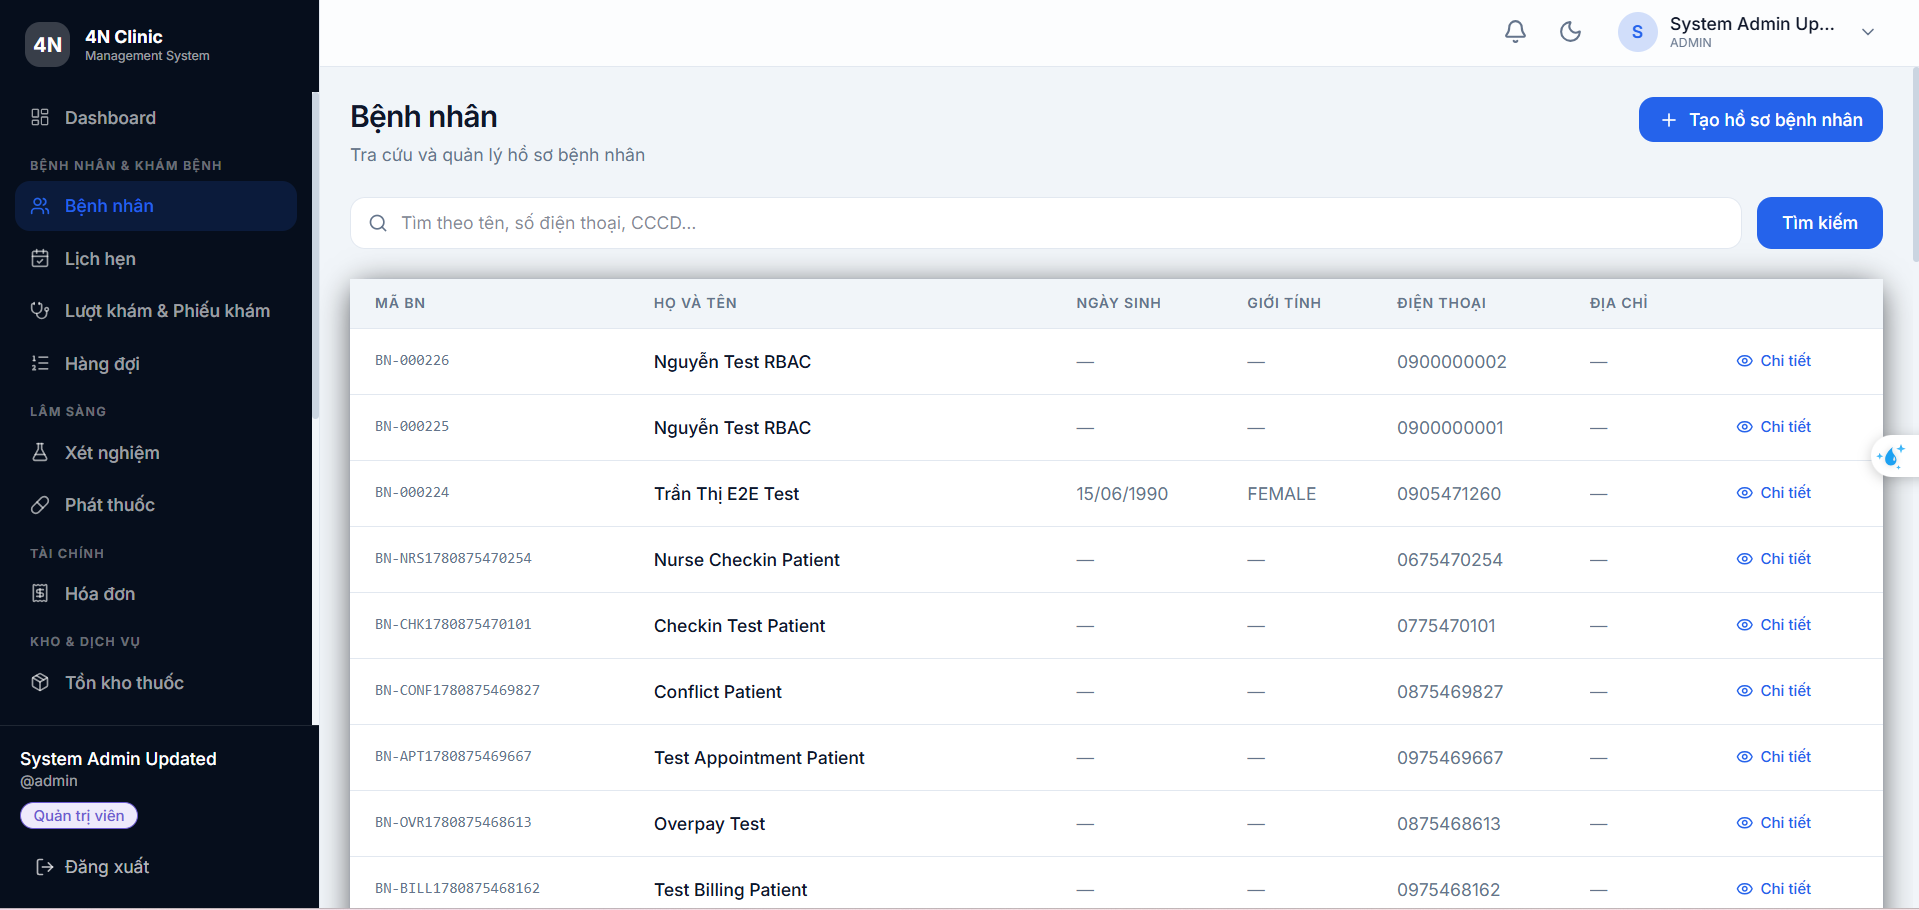
\includegraphics[width=0.8\textwidth]{figures/screenshots/patient-list.png}
    
    \caption*{(a) Danh sách bệnh nhân}
    
    \vspace{0.5cm}
    
    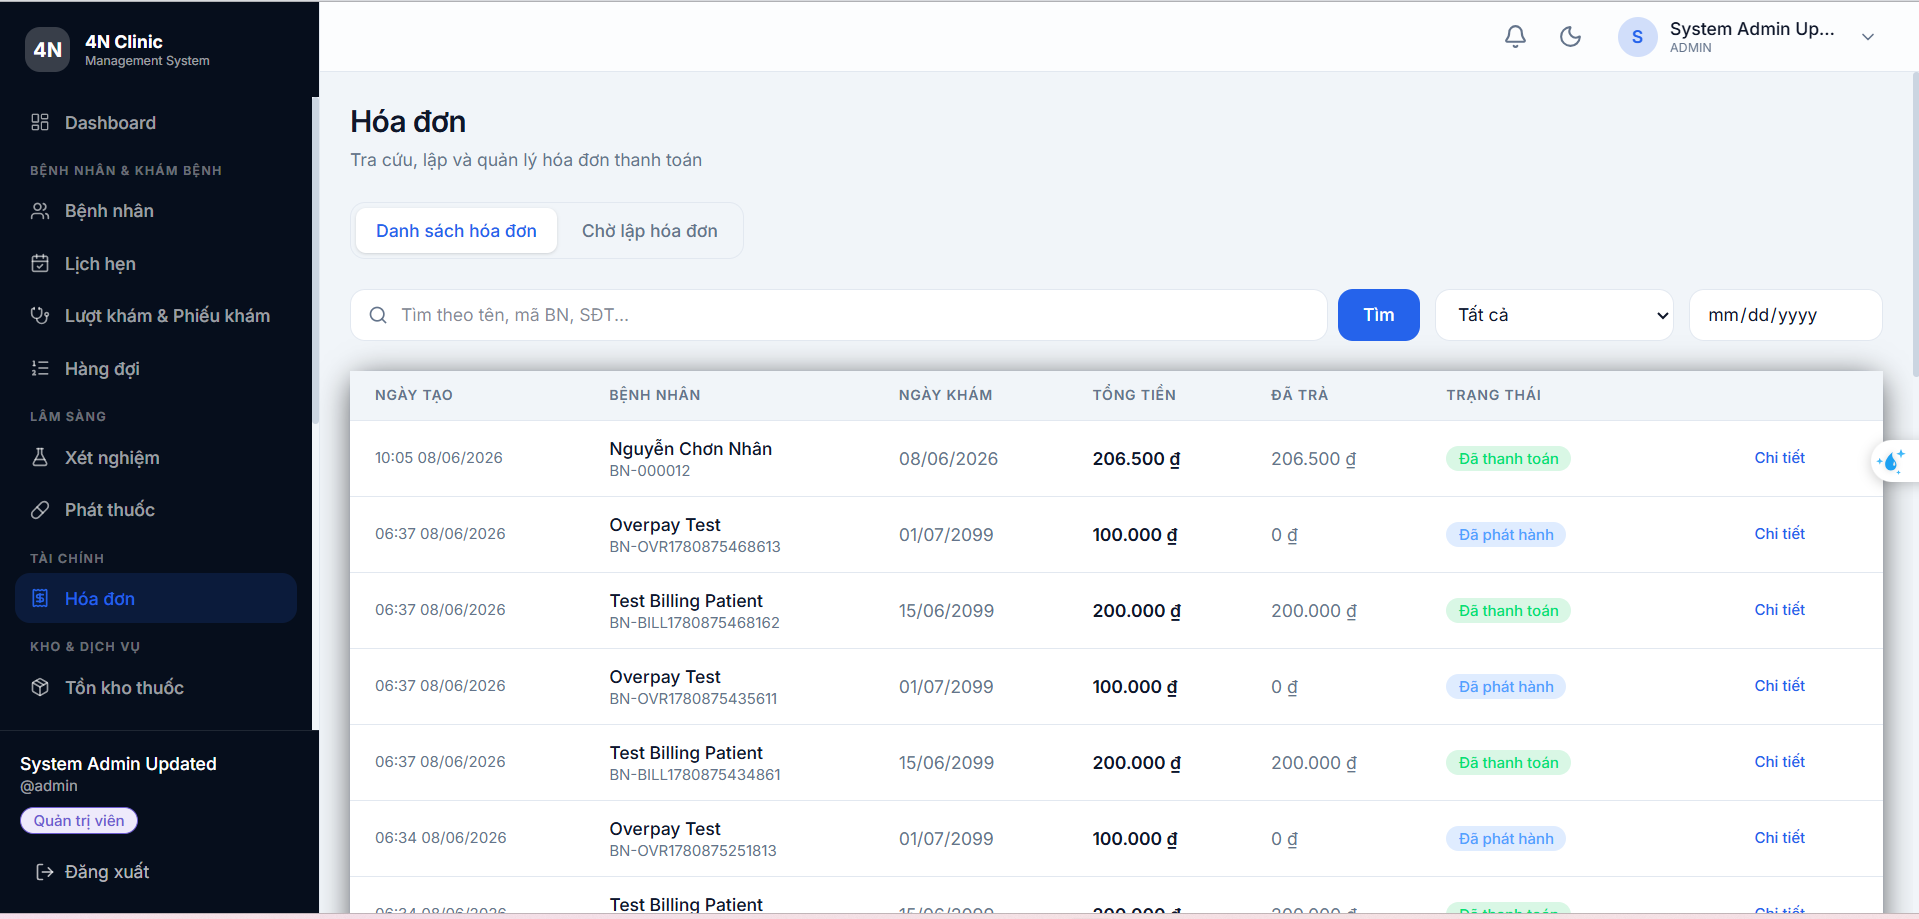
\includegraphics[width=0.8\textwidth]{figures/screenshots/invoice-detail.png}
    
    \caption*{(b) Chi tiết hóa đơn}
    
    \caption{Minh chứng giao diện cho hai nghiệp vụ quản lý bệnh nhân và thanh toán}
    \label{fig:ui-demo-patient-invoice}
\end{figure}
